\documentclass[conference]{IEEEtran}
\IEEEoverridecommandlockouts
\usepackage{cite}
\usepackage{amsmath,amssymb,amsfonts}
\usepackage{algorithmic}
\usepackage{graphicx}
\usepackage{textcomp}
\usepackage{xcolor}
\usepackage{booktabs}
\usepackage{multirow}
\def\BibTeX{{\rm B\kern-.05em{\sc i\kern-.025em b}\kern-.08em
    T\kern-.1667em\lower.7ex\hbox{E}\kern-.125emX}}
\begin{document}

\title{A Rate-Distortion Framework for Semantic Information: From Theory to Deep Learning}

\author{\IEEEauthorblockN{Wenlin Zhu, Yanqi Zhang}
\IEEEauthorblockA{\textit{School of Information Science and Technology} \\
\textit{ShanghaiTech University}\\
Shanghai, China \\
Email: \{zhuwl, zhangyq\}@shanghaitech.edu.cn}
}

\maketitle

\begin{abstract}
This paper presents a systematic study of the state-observation rate-distortion function (SORDF), a theoretical framework that jointly characterizes the tradeoff between semantic fidelity and appearance fidelity under a rate constraint. We reproduce the key theoretical results of the original framework across three canonical cases: the jointly Gaussian vector model, the binary classification model, and the joint rate-distortion setting with double constraints. We further extend the framework by incorporating ideas from task-oriented lossy compression with data, perception, and classification constraints \cite{wang2024task}, introducing a Rate-Distortion-Perception-Classification (RDPC) formulation for MNIST. Experiments on the MNIST dataset validate the tradeoff surfaces among reconstruction quality, perceptual realism, and classification accuracy under various rate budgets.
\end{abstract}

\begin{IEEEkeywords}
rate-distortion theory, semantic information, soft decision, perception constraint, deep learning
\end{IEEEkeywords}

\section{Introduction}

Shannon's classical rate-distortion theory provides the fundamental limits of lossy source coding, yet it does not account for semantic information. In many modern applications---from autonomous driving to medical imaging---the goal of communication is not merely to reproduce the raw signal, but to enable accurate inference at the receiver. This motivates a formal framework that jointly models both the semantic content and the observable appearance of a source.

The seminal work by Liu, Zhang, and Poor \cite{liu2021rate} proposed the state-observation rate-distortion function (SORDF), which decomposes a source into an unobservable intrinsic state $S$ (capturing semantics) and an observable extrinsic appearance $X$. The encoder observes only $X$, while the decoder must reconstruct both $\hat{S}$ and $\hat{X}$ under separate distortion constraints. This formulation reveals a counter-intuitive insight: locally optimal Bayesian classification followed by compression is strictly suboptimal compared to joint rate-distortion optimization.

In this project, we pursue two objectives. First, we provide a complete numerical reproduction of the key theoretical results from \cite{liu2021rate}, including the vector Gaussian case, the binary classification case with soft decision, and the achievable upper bound for joint constraints. Second, we extend the framework by incorporating a perception constraint through a Wasserstein GAN, formulating a Rate-Distortion-Perception-Classification (RDPC) problem, and validate it with deep learning experiments on MNIST.

\section{System Model and Problem Formulation}

\subsection{Source Model}

Consider a memoryless source characterized by a pair of random variables $(S, X) \sim p(s, x)$, where:
\begin{itemize}
    \item $S \in \mathcal{S}$ is the intrinsic state, representing the unobservable semantic content (e.g., class label, scene type);
    \item $X \in \mathcal{X}$ is the extrinsic observation, representing the observable appearance (e.g., pixel values, raw signal).
\end{itemize}

The encoder maps a length-$n$ block of observations $X^n$ to an index $W \in \{1, 2, \dots, 2^{nR}\}$, where $R$ is the coding rate in bits per source symbol. The decoder maps $W$ back to reconstructions $(\hat{S}^n, \hat{X}^n)$.

\subsection{Distortion Constraints and the SORDF}

Two distortion measures are defined:
\begin{itemize}
    \item \textbf{Semantic distortion}: $d_s(s, \hat{s})$, measuring the fidelity of the reconstructed semantic state;
    \item \textbf{Appearance distortion}: $d_a(x, \hat{x})$, measuring the fidelity of the reconstructed observation.
\end{itemize}

A rate-distortion triple $(R, D_s, D_a)$ is achievable if there exists a code of rate $R$ such that:
\begin{equation}
\lim_{n\to\infty} \mathbb{E}\, d_s(S^n, \hat{S}^n) \leq D_s, \quad
\lim_{n\to\infty} \mathbb{E}\, d_a(X^n, \hat{X}^n) \leq D_a.
\end{equation}

For one sample, the decoder output is generated only from the observation. Hence the Markov relation
$S \leftrightarrow X \leftrightarrow (\hat{S},\hat{X})$ holds for every admissible test channel. This allows the semantic distortion to be rewritten as
\begin{align}
\mathbb{E}[d_s(S,\hat{S})]
&= \sum_{x,\hat{s}} p(x)p(\hat{s}|x)
    \sum_s p(s|x)d_s(s,\hat{s}) \nonumber\\
&= \mathbb{E}[\hat{d}_s(X,\hat{S})],
\end{align}
where the equivalent semantic distortion is
\begin{equation}
\hat{d}_s(x, \hat{s}) = \mathbb{E}[d_s(S, \hat{s}) \mid X = x].
\label{eq:equiv-distortion}
\end{equation}
For continuous alphabets, the inner summation is replaced by the corresponding conditional integral. This step is important: although $S$ is never directly encoded, the distortion constraint can be evaluated through the posterior $p(s|x)$ induced by the observation.

The State-Observation Rate-Distortion Function  (SORDF) is therefore the infimum of achievable rates:
\begin{equation}
R(D_s, D_a) = \min_{p(\hat{s}, \hat{x}|x)} I(X; \hat{S}, \hat{X})
\label{eq:sordf}
\end{equation}
subject to $\mathbb{E}\,\hat{d}_s(X, \hat{S}) \leq D_s$ and $\mathbb{E}\,d_a(X, \hat{X}) \leq D_a$. The associated Lagrangian form is
\begin{equation}
\mathcal{L}=I(X;\hat{S},\hat{X})
 +\lambda_s \mathbb{E}[\hat{d}_s(X,\hat{S})]
 +\lambda_a \mathbb{E}[d_a(X,\hat{X})],
\label{eq:lazard}
\end{equation}
with $\lambda_s,\lambda_a\geq 0$. The numerical experiments in this report can be viewed as solving either the constrained problem in (\ref{eq:sordf}) directly or its Lagrangian dual form by sweeping the distortion multipliers. The special cases in the paper are valuable because they show how the optimal test channel differs from common engineering heuristics such as ``estimate the label first, then compress the label.''

\section{Case 1: Jointly Gaussian Vector Model}
\subsection{Theoretical Results}

Consider the specific task-oriented Gaussian vector model where the unobservable intrinsic semantic state $S \in \mathbb{R}$ is a scalar, and the observable appearance $X \in \mathbb{R}^m$ is an $m$-dimensional vector following \cite{liu2021rate}:
\begin{equation}
S \sim \mathcal{N}(0, \sigma_S^2), \quad
X = \mathbf{1}_m S + Z, \quad Z \sim \mathcal{N}(\mathbf{0}, \sigma_Z^2 \mathbf{I}_m),
\end{equation}
where $\mathbf{1}_m$ is an all-one vector of length $m$, and $S$ and the noise vector $Z$ are mutually independent. Both semantic and appearance distortions are measured by the squared errors: $d_s(s, \hat{s}) = (s - \hat{s})^2$ and $d_a(x, \hat{x}) = \|x - \hat{x}\|^2$, respectively.

For a squared semantic error, the optimal reconstruction of $S$ from any representation of $X$ is given by its conditional mean. We define the minimum mean-square error (MMSE) estimator as:
\begin{equation}
\tilde{S}(X) = \mathbb{E}[S|X] = \frac{\sigma_S^2}{m\sigma_S^2 + \sigma_Z^2} \mathbf{1}_m^T X.
\end{equation}
By invoking the orthogonality principle of MMSE estimation, the expected semantic distortion can be decoupled as:
\begin{align}
\mathbb{E}[(S-\hat{S})^2]
&=\mathbb{E}[(S-\tilde{S}(X))^2] + \mathbb{E}[(\tilde{S}(X)-\hat{S})^2] \nonumber\\
&=\text{mmse} + \mathbb{E}[(\tilde{S}(X)-\hat{S})^2],
\label{eq:orthogonal}
\end{align}
where the irreducible estimation error is
\begin{equation}
\text{mmse} = \frac{\sigma_S^2 \sigma_Z^2}{m\sigma_S^2 + \sigma_Z^2}.
\label{eq:gaussian-mmse}
\end{equation}
This formulation shows that the semantic constraint is equivalent to compressing the MMSE estimator $\tilde{S}(X)$ with a remaining distortion budget $D_s-\mathrm{mmse}$.

For the symmetric vector model, the paper diagonalizes the covariance into one semantic direction and $m-1$ orthogonal observation-only directions \cite{liu2021rate}. It is useful to define:
\begin{equation}
\alpha^2=\frac{(m\sigma_S^2+\sigma_Z^2)^2}{m\sigma_S^2}.
\end{equation}
The semantic constraint becomes a water-filling constraint on the first eigen-direction with a budget of $B=\alpha^2(D_s-\mathrm{mmse})$, while the appearance constraint allocates distortion across the same first direction and the remaining $m-1$ noise directions. This joint allocation is what creates the five-region phase diagram.

Let $\lambda_1=m\sigma_S^2+\sigma_Z^2$, $\lambda_2=\sigma_Z^2$, and $B=\alpha^2(D_s-\mathrm{mmse})$. Proposition 4 of \cite{liu2021rate} gives the closed-form SORDF over five regions:
\begin{equation}
R(D_s, D_a) = 
\begin{cases}
\frac{1}{2}\log_2\frac{\lambda_1}{B} + \frac{m-1}{2}\log_2\frac{(m-1)\lambda_2}{D_a-B}, & \text{for } (D_s, D_a) \in S_1, \\
\frac{1}{2}\log_2\frac{m\lambda_1}{D_a} + \frac{m-1}{2}\log_2\frac{m\lambda_2}{D_a}, & \text{for } (D_s, D_a) \in S_2, \\
\frac{1}{2}\log_2\frac{\lambda_1}{B}, & \text{for } (D_s, D_a) \in S_3, \\
\frac{1}{2}\log_2\frac{\lambda_1}{D_a-(m-1)\lambda_2}, & \text{for } (D_s, D_a) \in S_4, \\
0, & \text{for } (D_s, D_a) \in S_5,
\end{cases}
\label{eq:sordf_gaussian}
\end{equation}
where the five geometric regions are defined as follows:
\begin{itemize}
    \item \textbf{Region $S_1$ (Joint active region):} $D_s \ge \text{mmse}$ and $m B \le D_a \le B + (m-1)\sigma_Z^2$.
    \item \textbf{Region $S_2$ (Low-distortion appearance dominated):} $0 \le D_a < m\sigma_Z^2$ and $B \ge D_a / m$.
    \item \textbf{Region $S_3$ (Semantic dominated):} $0 \le B < m\sigma_S^2 + \sigma_Z^2$ and $D_a > B + (m-1)\sigma_Z^2$.
    \item \textbf{Region $S_4$ (High-distortion appearance dominated):} $m\sigma_Z^2 \le D_a < m\sigma_S^2 + m\sigma_Z^2$ and $B \ge D_a - (m-1)\sigma_Z^2$.
    \item \textbf{Region $S_5$ (Unconstrained zero-rate):} $D_a \ge m\sigma_S^2 + m\sigma_Z^2$ and $B \ge m\sigma_S^2 + \sigma_Z^2$.
\end{itemize}
Intuitively, $S_1$ is the truly joint region where both semantic and appearance constraints are active; $S_2$ and $S_4$ are dominated by appearance coding; $S_3$ is dominated by semantic coding; and $S_5$ is the zero-rate region.
\subsection{Numerical Reproduction}

We implemented the complete piecewise formula for the vector Gaussian case and used the same normalized parameters $m=3$, $\sigma_S^2=1$, $\sigma_Z^2=1$ for the five-region illustration. With these values, $\mathrm{mmse}=0.25$ and $\alpha^2=16/3$, so the visible intersection of the two slanted boundaries is at $D_s=\mathrm{mmse}+\sigma_Z^2/\alpha^2=0.4375$. Fig.~\ref{fig:fig2} shows the resulting partition of the $(D_s,D_a)$ plane.

\begin{figure}[htbp]
\centerline{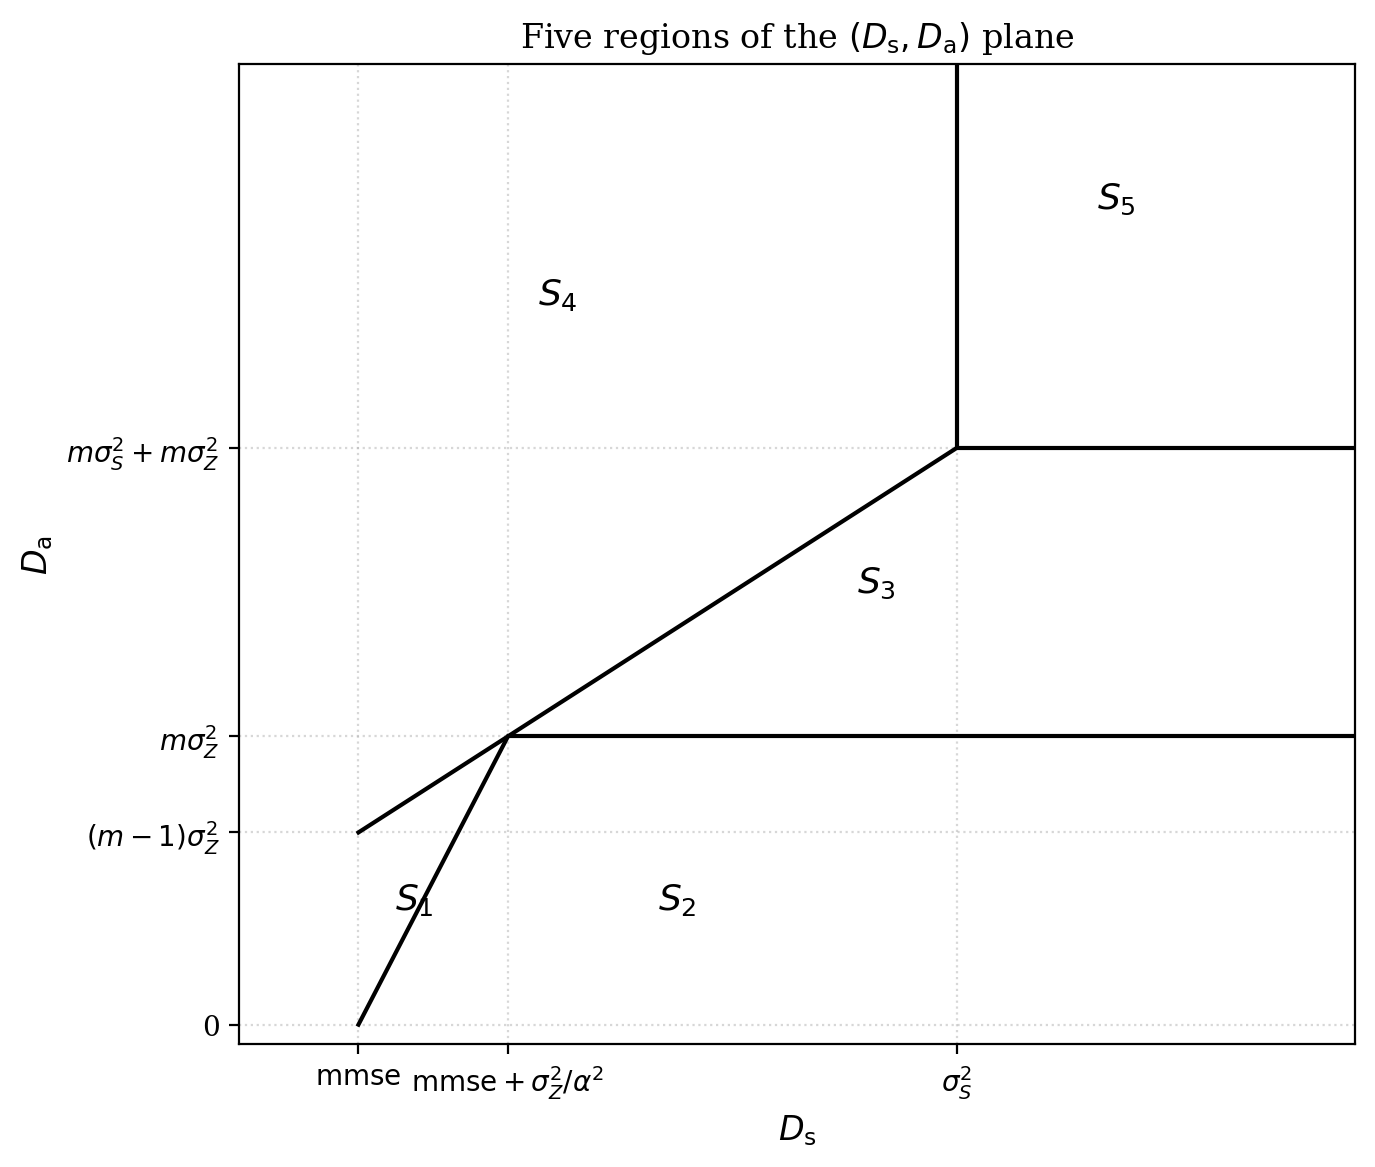
\includegraphics[width=\columnwidth]{../rd-semantic-repro/figures/fig2_five_regions.png}}
\caption{Illustration of the five regions of the $(D_s, D_a)$ plane for the jointly Gaussian vector model ($m=3$, $\sigma_S^2=1$, $\sigma_Z^2=1$).}
\label{fig:fig2}
\end{figure}

Fig.~\ref{fig:fig3} displays the 3D surface and contour plot of $R(D_s, D_a)$. The surface exhibits distinct behaviors: in region $S_5$, zero rate is achievable when both distortion constraints are sufficiently loose; in regions $S_1$ through $S_4$, the rate increases as the constraints tighten, with different functional forms in each region.

\begin{figure}[htbp]
\centerline{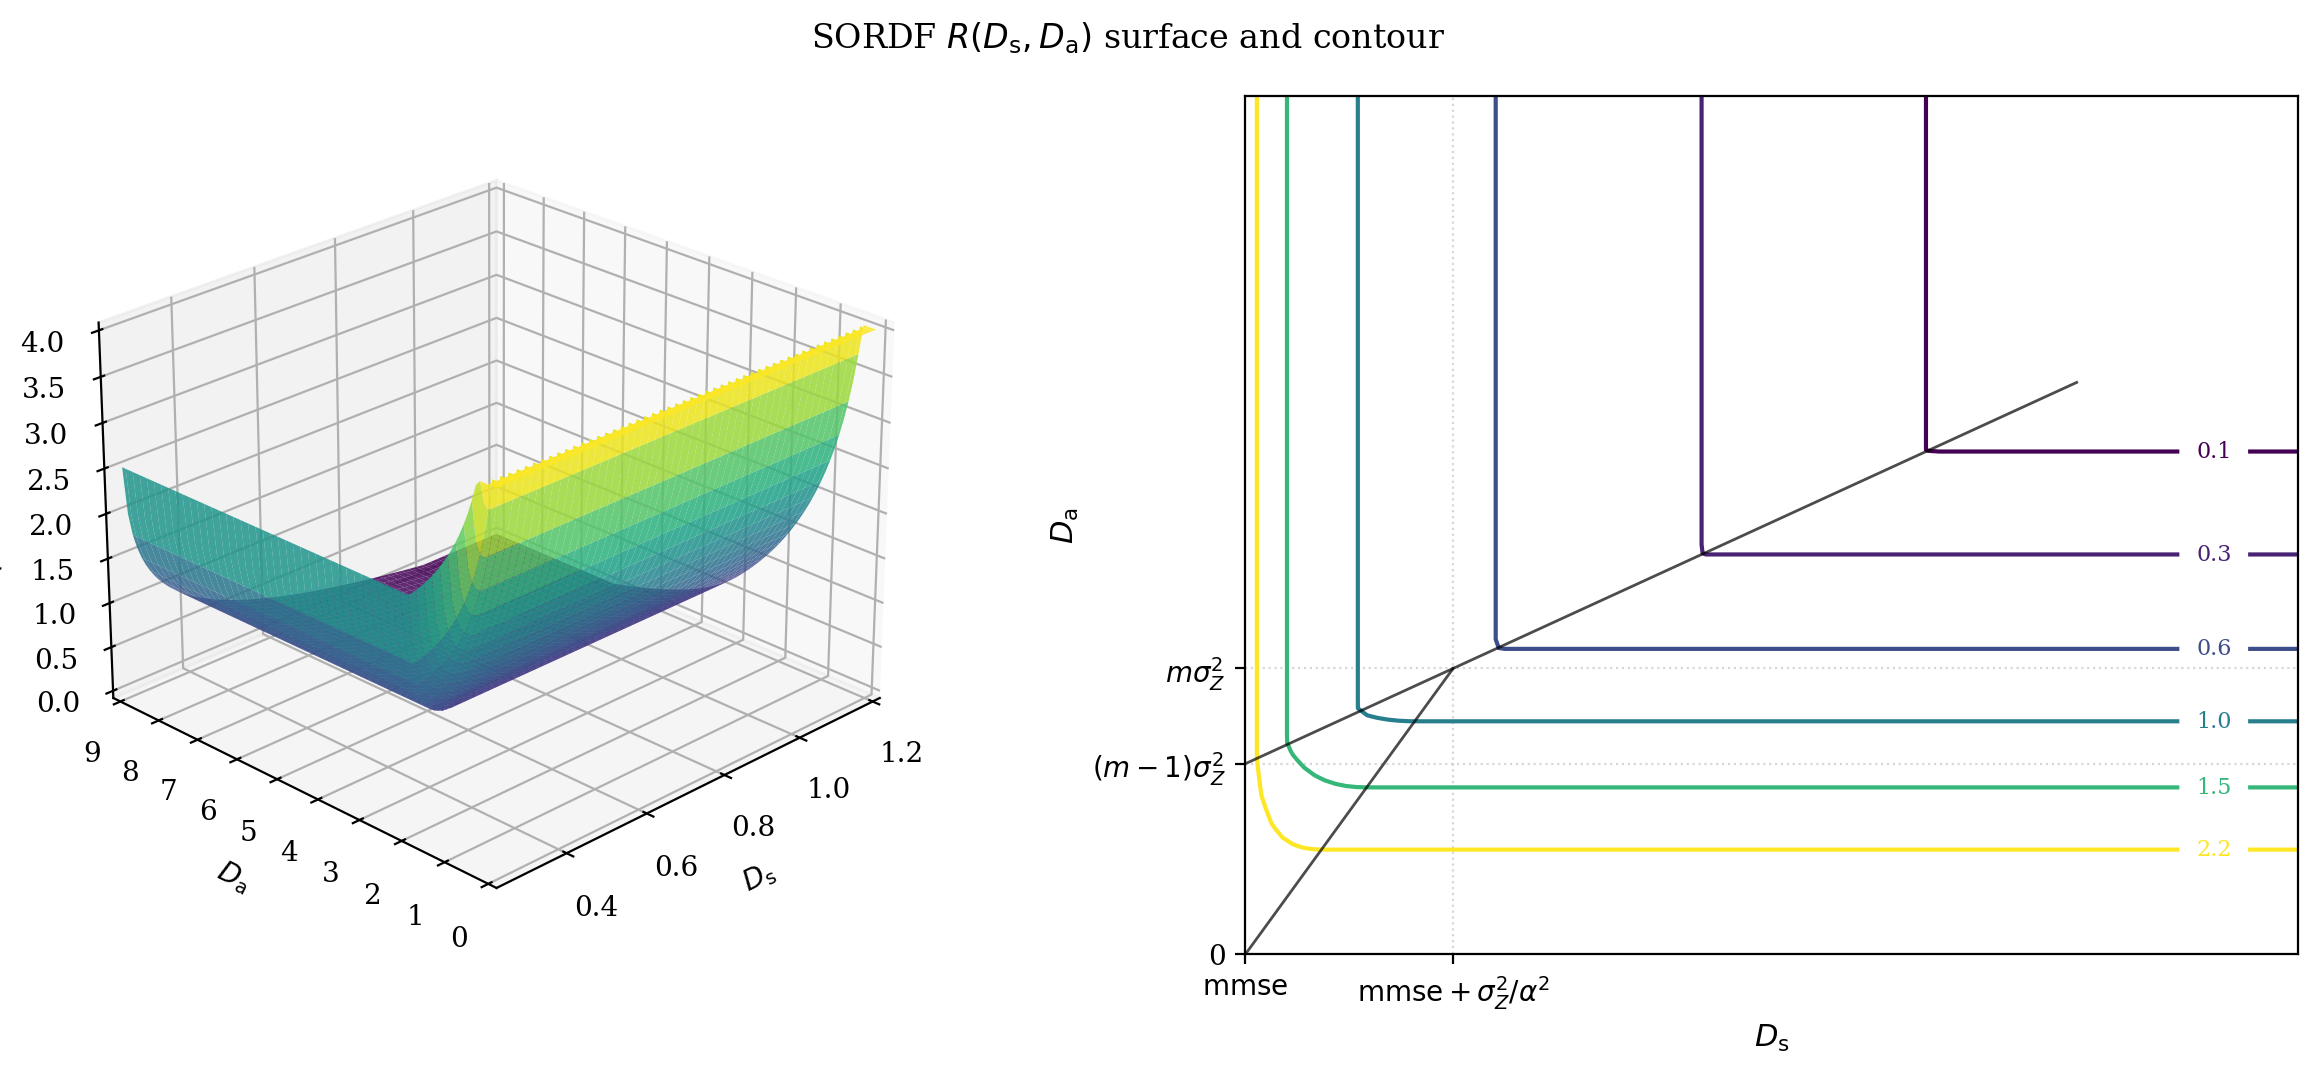
\includegraphics[width=\columnwidth]{../rd-semantic-repro/figures/fig3_sordf_3d_contour.png}}
\caption{The SORDF $R(D_s, D_a)$ as a 3D surface (left) and its contour plot (right).}
\label{fig:fig3}
\end{figure}

\section{Case 2: Binary Classification with Soft Decision}

\subsection{Problem Setup}

In the binary classification case, the semantic state $S$ is a binary label with uniform prior, and the observation $X$ is conditionally Gaussian:
\begin{align}
S &\sim \text{Bernoulli}(1/2),\\
X|S=0 &\sim \mathcal{N}(A, \sigma^2),\\
X|S=1 &\sim \mathcal{N}(-A, \sigma^2).
\end{align}
Semantic distortion is Hamming distance (classification error rate), and we first consider unconstrained appearance ($D_a = \infty$).

\subsection{Soft vs. Hard Decision}

The posterior probability of class $S=0$ is
\begin{equation}
p(0|x)=\frac{N^+(x)}{N^+(x)+N^-(x)}
       =\frac{1}{1+\exp(-2Ax/\sigma^2)},
\label{eq:posterior}
\end{equation}
where $N^+(x)$ and $N^-(x)$ are the conditional Gaussian densities centered at $A$ and $-A$. The Bayes classifier thresholds $x$ at zero and achieves error
\begin{equation}
P_e^*=Q(A/\sigma).
\end{equation}
This is the smallest possible semantic distortion if the decoder must output a hard label. However, the rate-distortion problem is different: 
The optimal test channel allows a randomized reconstruction,
described by the conditional probability
\[
g(x)=P(\hat S=0|X=x),
\]
rather than making a deterministic MAP decision.

Let $g(x)=p(\hat{S}=0|X=x)$. For Hamming distortion, the expected semantic distortion contributed by a sample $x$ is
\begin{align}
\hat{d}_s(x,0)&=p(1|x),\\
\hat{d}_s(x,1)&=p(0|x).
\end{align}
The state-observation rate-distortion problem seeks the conditional distribution
$g(x)=P(\hat{S}=0|X=x)$
that minimizes the mutual information
$I(X;\hat{S})$
subject to the semantic distortion constraint and the symmetry condition
$\Pr(\hat{S}=0)=1/2$.
By introducing a Lagrange multiplier for the distortion constraint and solving the resulting variational optimization problem, Proposition~5 shows that the optimal reconstruction is not a hard classifier but a soft probabilistic mapping:
\begin{equation}
g(x) = \left[1 + \exp\left(\lambda \frac{1 - e^{-2Ax/\sigma^2}}{1 + e^{-2Ax/\sigma^2}}\right)\right]^{-1},
\end{equation}
where $\lambda < 0$ is a Lagrange multiplier chosen to satisfy the distortion constraint
\begin{equation}
\int_{-\infty}^{\infty} [N^+(x)-N^-(x)]g(x)\,dx=1-2D_s.
\label{eq:lambda-binary}
\end{equation}
The optimal rate is:
\begin{equation}
R(D_s, \infty) = 1 - \frac{1}{2}\int_{-\infty}^{\infty} [N^+(x) + N^-(x)]\, h_2(g(x))\, dx,
\end{equation}
where $N^+(x)$ and $N^-(x)$ are the conditional Gaussian densities, and $h_2(\cdot)$ is the binary entropy function.

The key observation is that the conventional pipeline of first performing Bayes classification and then compressing the resulting binary label is generally suboptimal. Such a strategy discards the confidence information contained in the observation $x$, retaining only its sign. In contrast, the optimal test channel preserves this confidence through the soft reconstruction probability $g(x)$. Samples far from the decision boundary are reconstructed almost deterministically, whereas ambiguous samples near $x=0$ are assigned probabilities close to $1/2$. Consequently, semantic compression should jointly optimize inference and compression instead of separating them into independent stages.

\subsection{Numerical Results}

Fig.~\ref{fig:fig4} and Fig.~\ref{fig:fig4b} present the key results for $A=1$ and $\sigma=1$. The left panel shows the soft decision function $g(x)$ under four different semantic distortion targets. As $D_s$ approaches the Bayes error $Q(A/\sigma) \approx 0.1587$, the multiplier magnitude grows and $g(x)$ approaches a hard step function. As $D_s \to 0.5$, $\lambda\to 0$ and $g(x)$ flattens to $0.5$, indicating that no information about $S$ is preserved.

The right panel compares the rate-distortion curves of the optimal soft decision scheme versus the naive hard-decision-then-compress scheme. The gap between the two curves quantifies the benefit of joint optimization: the soft decision approach achieves strictly lower rates for the same semantic distortion, except at the extreme point $D_s = Q(A/\sigma)$ where both coincide.

\begin{figure}[htbp]
\centerline{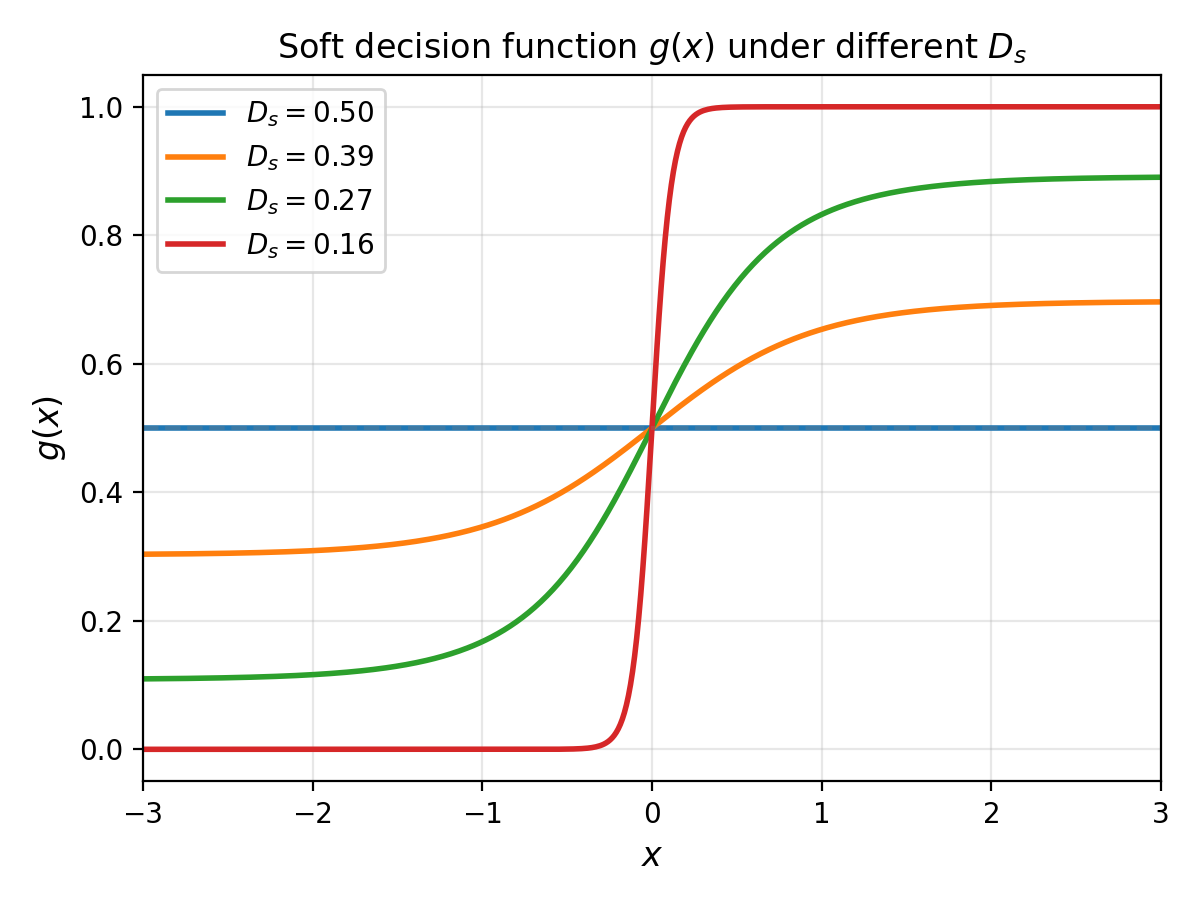
\includegraphics[width=\columnwidth]{../rd-semantic-repro/figures/fig4_left_gx.png}}
\caption{Left: Soft decision function $g(x)$ under different $D_s$. Right: Rate-distortion comparison between optimal soft decision and naive hard decision schemes ($A=1$, $\sigma=1$).}
\label{fig:fig4}
\end{figure}

\begin{figure}[htbp]
\centerline{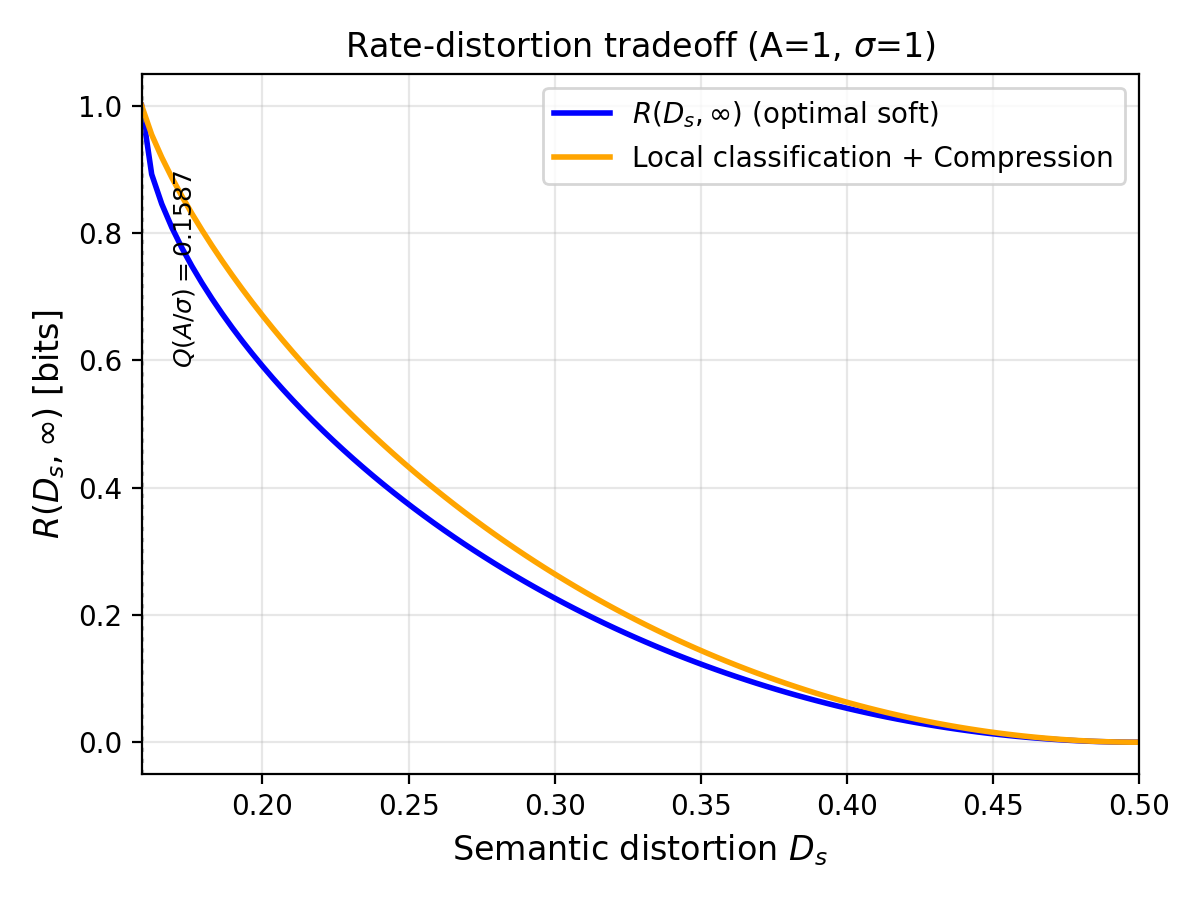
\includegraphics[width=\columnwidth]{../rd-semantic-repro/figures/fig4_right_rd.png}}
\caption{Rate-distortion tradeoff: optimal soft decision vs.\ naive hard-decision-then-compress.}
\label{fig:fig4b}
\end{figure}

\section{Case 3: Joint Rate-Distortion with Double Constraints}

\subsection{Achievable Upper Bound}

When both semantic and appearance constraints are active, Proposition 6 of \cite{liu2021rate} provides an achievable upper bound via a two-stage coding scheme. This case is important because the optimal binary semantic code alone does not necessarily preserve enough information to reconstruct the observation $X$. The construction separates the total rate into a semantic part and a conditional appearance-refinement part.

Stage 1 chooses an intermediate semantic distortion $D$ satisfying
\begin{equation}
Q(A/\sigma)\leq D\leq D_s
\label{eq:D_feasible}
\end{equation}
and encodes the soft semantic decision using the $R(D,\infty)$ construction from Case 2. This produces a reproduction variable $\hat{S}$ that satisfies the semantic constraint but leaves an observation residual. Stage 2 encodes the residual 
\begin{equation}
X - \mathbb{E}[X \mid \hat{S}]
\label{eq:residual}
\end{equation}
conditioned on the semantic reconstruction $\hat{S}$ using a Gaussian rate-distortion code. The value of $D$ is optimized because a stricter semantic first stage can reduce the appearance residual but costs more semantic bits.

For a fixed $D$, let $\lambda(D)$ solve (\ref{eq:lambda-binary}) and let
\begin{align}
\gamma(D) &= \int_{-\infty}^{\infty} x \, [N^+(x) + N^-(x)] g_D(x) \, dx, \label{eq:gamma_def} \\
\eta(D) &= \int_{-\infty}^{\infty} (x - \gamma(D))^2 \, [N^+(x) + N^-(x)] g_D(x) \, dx. \label{eq:eta_def}
\end{align}
Here, $\gamma(D)$ denotes the conditional mean of the observation associated with the semantic reconstruction, while $\eta(D)$ is the corresponding residual variance left for appearance coding. The appearance refinement then costs
\begin{equation}
\frac{1}{2} \left( \log_2 \frac{\eta(D)}{D_a} \right)^+,
\label{eq:refinement_cost}
\end{equation}
where $(x)^+ \triangleq \max\{x, 0\}$.

The achievable rate is:
\begin{equation}
R_{\text{ach}}(D_s, D_a) = \min_{D \in [Q(A/\sigma), D_s]} \left[ R(D, \infty) + \frac{1}{2}\left(\log_2 \frac{\eta(D)}{D_a}\right)^+ \right].
\label{eq:rach_def}
\end{equation}
Unlike Proposition 4 and Proposition 5, Proposition 6 does not characterize the exact SORDF. Instead, it constructs a feasible two-stage coding strategy whose achievable rate serves as an upper bound on the optimal state-observation rate-distortion function.

\subsection{Numerical Results}

The reproduction numerically evaluates the achievable upper bound in (\ref{eq:rach_def}) by discretizing the candidate semantic distortion $D$ over its feasible interval and computing the corresponding rate for each candidate. Following the setup in Figure 6 of the original paper, Fig.~\ref{fig:fig5} shows the achievable upper-bound curves for three semantic distortion targets ($D_s = 0.50, 0.30, 0.10$) with $A^2/\sigma^2 = 10$. Two baselines are also plotted: direct encoding of $X$ while ignoring semantics, and the ideal case where $S$ is known exactly before appearance coding.

As $D_s$ decreases (stricter semantic requirement), the rate increases for all appearance distortion levels. As the appearance distortion constraint becomes tighter, more bits are required to refine the observation conditioned on the semantic reconstruction. Consequently, the achievable rate gradually transitions from semantic-dominated coding to appearance-dominated coding.

\section{Extension: RDPC Framework on MNIST}

\subsection{From SORDF to RDPC}

The original paper studies two objectives:

1. semantic distortion

2. appearance distortion

However, modern image generation research has shown that
pixel-wise distortion alone is insufficient to characterize
visual quality.
Images with low MSE are often blurry although semantically
correct.

Therefore,
we introduce an additional perception constraint,
leading to the proposed
Rate-Distortion-Perception-Classification (RDPC) framework.

\subsection{Motivation and Formulation}

The original SORDF framework uses an appearance distortion such as pixel-wise MSE. This is mathematically convenient, but in image compression it often produces blurry reconstructions: the conditional mean minimizes MSE even when it is not a realistic image. Inspired by perception-constrained compression \cite{blau2019rethinking} and the task-oriented lossy compression framework with data, perception, and classification constraints \cite{wang2024task}, we introduce a third constraint---perceptual quality---and an explicit classification constraint into the semantic rate-distortion framework.

We formulate the \textbf{Rate-Distortion-Perception-Classification (RDPC)} problem:
\begin{equation}
R(D, P, C) = \min_{p(\hat{x}|x)} I(X; \hat{X})
\end{equation}
subject to:
\begin{align}
\mathbb{E}[\Delta(X, \hat{X})] &\leq D \quad \text{(Reconstruction)} \\
d_{\text{W}}(p_X, p_{\hat{X}}) &\leq P \quad \text{(Perception)} \\
H(S \mid \hat{X}) &\leq C \quad \text{(Classification)}
\end{align}
where $d_{\text{W}}$ is the Wasserstein distance and $H(S \mid \hat{X})$ bounds the classification uncertainty.
Compared with the original SORDF, $S$ is no longer reconstructed as an explicit symbol. Instead, the semantic constraint is imposed by requiring a classifier applied to $\hat{X}$ to retain the label information. This is natural for MNIST: if a reconstruction is visually plausible but changes a ``3'' into an ``8'', it has good perception but poor semantic fidelity.

\subsection{Deep Learning Architecture}

We implement the RDPC framework using a deep autoencoder with three learning objectives, as shown in Fig.~\ref{fig:arch}. The encoder maps an image to a low-dimensional latent vector; the decoder reconstructs an image; a WGAN-GP critic estimates the perception term; and a frozen classifier measures whether the reconstructed image preserves the semantic label.

\begin{figure}[htbp]
\centerline{\includegraphics[width=\columnwidth]{../rdpc_mnist/results/rdpc_architecture.png}}
\caption{RDPC training pipeline. The latent dimension $k$ controls the rate proxy; MSE, WGAN-GP, and classifier losses implement the distortion, perception, and semantic constraints.}
\label{fig:arch}
\end{figure}

The implemented modules are:
\begin{itemize}
    \item \textbf{Encoder}: CNN mapping $X \in \mathbb{R}^{28\times28}$ to latent $Z \in \mathbb{R}^k$ (rate controlled by latent dimension $k$);
    \item \textbf{Decoder}: Transposed CNN reconstructing $\hat{X}$ from $Z$;
    \item \textbf{Discriminator}: WGAN-GP critic enforcing the perception constraint via gradient penalty;
    \item \textbf{Classifier}: Pre-trained frozen CNN providing semantic supervision on $\hat{X}$.
\end{itemize}

The joint training loss is:
\begin{equation}
\mathcal{L}_{G} = \lambda_d \cdot \text{MSE}(x, \hat{x})
 - \lambda_p \cdot D_\psi(\hat{x})
 + \lambda_c \cdot \text{CE}(s, C(\hat{x})),
\label{eq:rdpc-loss}
\end{equation}
where $D_\psi(\hat{x})$ is the critic score (higher means more realistic), $C(\cdot)$ is the frozen classifier, and CE is cross-entropy loss. The critic is trained with
\begin{equation}
\mathcal{L}_{D}=D_\psi(\hat{x})-D_\psi(x)
 +\lambda_{\mathrm{gp}}\mathbb{E}_{\bar{x}}
 \left(\|\nabla_{\bar{x}}D_\psi(\bar{x})\|_2-1\right)^2,
\end{equation}
where $\bar{x}$ is a random interpolation between real and reconstructed images. This WGAN-GP term approximates the Wasserstein perception constraint in the Lagrangian form.

The true mutual information $I(X;Z)$ is difficult to estimate in a neural model. We therefore use a Gaussian entropy upper-bound proxy:
\begin{equation}
\hat{R}(Z)=\frac{1}{2}\sum_{i=1}^{k}\log_2(1+\widehat{\mathrm{Var}}[Z_i]).
\label{eq:rate-proxy}
\end{equation}
This proxy is not an exact operational coding rate, but it is useful for comparing configurations: increasing $k$ or increasing latent variance generally increases $\hat{R}$.

\subsection{Experimental Protocol}

The implemented experimental procedure consists of four steps:
\begin{enumerate}
    \item Train a CNN classifier on clean MNIST images for 5 epochs and freeze it. This classifier supplies the semantic loss in (\ref{eq:rdpc-loss}).
    \item For each configuration $(k,\lambda_p,\lambda_c)$, train the RDPC autoencoder with $\lambda_d=1$, WGAN-GP weight $\lambda_{\mathrm{gp}}=10$, and $n_{\mathrm{critic}}=5$ critic updates per generator update.
    \item Evaluate each checkpoint on the MNIST test set using three metrics: rate proxy $\hat{R}$, reconstruction MSE, and classifier accuracy on reconstructed images.
    \item Plot the resulting tradeoffs: rate-distortion, rate-classification, distortion-classification, and the effect of the Lagrange weights at fixed latent dimension.
\end{enumerate}

The full sweep intended for the extension is
\begin{align}
k&\in\{4,8,16,32,64\},\\
\lambda_p&\in\{0.01,0.1,1.0\},\\
\lambda_c&\in\{0.1,1.0,10.0\}.
\end{align}
This gives 45 configurations. Because full training is expensive, the current report includes a representative subset and provides the scripts needed to reproduce the complete sweep.

\subsection{Experimental Results}

Table~\ref{tab:sweep} presents representative RDPC results. The results are not yet a full 45-point sweep; rather, they are selected configurations that cover low, medium, and high rate regimes and several perception/classification weight settings.

\begin{table}[htbp]
\caption{Representative RDPC results on MNIST.}
\begin{center}
\begin{tabular}{cccccc}
\toprule
$k$ & $\lambda_p$ & $\lambda_c$ & Rate (bits) & MSE & Acc (\%) \\
\midrule
4  & 0.01 & 0.1  & 9.50  & 31.52 & 98.01 \\
4  & 1.0  & 10.0 & 10.64 & 54.90 & 97.85 \\
16 & 0.01 & 1.0  & 41.67 & 33.44 & 98.98 \\
16 & 0.1  & 1.0  & 42.22 & 24.27 & 98.24 \\
16 & 1.0  & 10.0 & 41.64 & 36.61 & 97.76 \\
32 & 0.1  & 1.0  & 81.25 & 19.41 & 98.45 \\
64 & 0.1  & 0.1  & 180.0 & 12.21 & 98.15 \\
\bottomrule
\end{tabular}
\label{tab:sweep}
\end{center}
\end{table}

\begin{figure}[htbp]
\centerline{\includegraphics[width=\columnwidth]{../rdpc_mnist/results/rdpc_tradeoffs.png}}
\caption{Representative RDPC tradeoff plots: rate-distortion, rate-classification, and distortion-classification.}
\label{fig:rdpc-tradeoffs}
\end{figure}

\begin{figure}[htbp]
\centerline{\includegraphics[width=\columnwidth]{../rdpc_mnist/results/rdpc_lambda_effects.png}}
\caption{Sparse RDPC Lagrange-weight sensitivity at fixed latent dimension. Left: perception-weight effect on MSE for the available $k=16,\lambda_c=1$ points. Right: representative $k=16$ operating points under different $(\lambda_p,\lambda_c)$ settings.}
\label{fig:rdpc-lambda}
\end{figure}

Several observations emerge:
\begin{enumerate}
    \item \textbf{Rate-dimension relationship}: The estimated rate increases with latent dimension $k$, consistent with the Gaussian entropy proxy in (\ref{eq:rate-proxy}). Moving from $k=4$ to $k=64$ increases the rate proxy from roughly 10 bits to 180 bits.
    \item \textbf{Distortion-rate behavior}: Higher latent dimension generally reduces MSE. The representative high-rate configuration $k=64$ has MSE 12.21, while the low-rate $k=4$ configurations have MSE above 31.
    \item \textbf{Classification robustness}: The classification accuracy remains above 97\% for all representative configurations in Table~\ref{tab:sweep}, demonstrating that semantic information can be preserved even when the reconstruction MSE varies substantially.
    \item \textbf{Three-way tradeoff}: At fixed rate (e.g., $k=16$), varying $(\lambda_p, \lambda_c)$ traces a two-dimensional tradeoff surface. Higher $\lambda_p$ pushes reconstructions toward the data manifold through the critic, while higher $\lambda_c$ pushes them toward classifier-stable semantic content. These objectives can conflict with pixel MSE.
\end{enumerate}

\section{Implementation and Testing Methodology}

All theoretical computations are implemented in Python using NumPy, SciPy, and Matplotlib. The SORDF computations involve:
\begin{itemize}
    \item Numerical integration via adaptive quadrature (\texttt{scipy.integrate.quad});
    \item Root-finding for the Lagrange multiplier $\lambda$ via Brent's method (\texttt{scipy.optimize.brentq});
    \item Gaussian Q-function and binary entropy function implementations.
\end{itemize}

The codebase follows a test-driven development approach. Each theorem-level claim from the paper is encoded as a boundary-condition test:
\begin{itemize}
    \item $D_s < Q(A/\sigma)$ is infeasible (raises \texttt{ValueError});
    \item At $D_s = Q(A/\sigma)$, the rate equals 1 bit;
    \item At $D_s = 0.5$, the rate is zero;
    \item Better class separation (larger $A/\sigma$) reduces the minimum achievable $D_s$;
    \item The rate function is monotone non-increasing in $D_s$.
\end{itemize}

The deep learning pipeline uses PyTorch with a WGAN-GP training regime. The discriminator is updated $n_{\text{critic}} = 5$ times per generator update, with gradient penalty weight $\lambda_{\text{gp}} = 10$. The classifier is pre-trained for 5 epochs on clean MNIST images and frozen during RDPC training.

\section{Conclusion}

This project provides a comprehensive reproduction and extension of the rate-distortion framework for semantic information. On the theoretical side, we numerically validated the SORDF across three canonical cases: the vector Gaussian model with its five-region phase diagram, the binary classification model revealing the optimality of soft decision over hard Bayesian classification, and the joint constraint setting with an achievable two-stage coding bound.

On the practical side, we extended the framework to include a perception constraint via WGAN-GP, formulating the RDPC problem. Deep learning experiments on MNIST demonstrate the feasibility of simultaneously optimizing for reconstruction quality, perceptual realism, and classification accuracy, and reveal the rich tradeoff surfaces among these three objectives under rate constraints.

Future work includes developing neural estimators for the SORDF that can operate on high-dimensional data without closed-form solutions, extending the RDPC framework to more complex datasets (e.g., CIFAR-10, ImageNet), and investigating whether the soft-decision optimality result generalizes to deep learning-based semantic communication systems.

\begin{thebibliography}{00}
\bibitem{liu2021rate} J. Liu, W. Zhang, and H. V. Poor, ``A rate-distortion framework for characterizing semantic information,'' in \textit{Proc. IEEE Int. Symp. Inf. Theory (ISIT)}, 2021.
\bibitem{blau2019rethinking} Y. Blau and T. Michaeli, ``Rethinking lossy compression: The rate-distortion-perception tradeoff,'' in \textit{Proc. Int. Conf. Mach. Learn. (ICML)}, 2019.
\bibitem{wang2024task} Y. Wang, Y. Wu, S. Ma, and Y.-J. A. Zhang, ``Task-oriented lossy compression with data, perception, and classification constraints,'' arXiv preprint arXiv:2405.04144, 2024.
\bibitem{cover2006elements} T. M. Cover and J. A. Thomas, \textit{Elements of Information Theory}, 2nd ed. Wiley, 2006.
\bibitem{shannon1959coding} C. E. Shannon, ``Coding theorems for a discrete source with a fidelity criterion,'' \textit{IRE Nat. Conv. Rec.}, vol. 7, pp. 142--163, 1959.
\end{thebibliography}

\end{document}
